%!TEX root = ../Physik I.tex

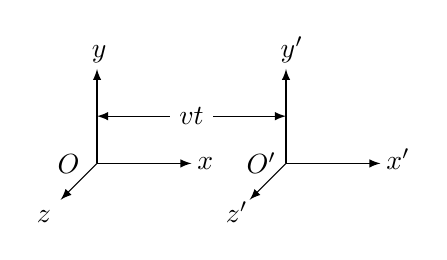
\begin{tikzpicture}[>=latex,scale=1.2]
	\begin{scope}
		\draw[->] (0,0) -- (xyz cs:x=1) node[right,xshift=-.5mm,yshift=.5mm]{$x\phantom{'}$};
		\draw[->] (0,0) -- (xyz cs:y=1) node[above,xshift=.75mm,yshift=-.5mm]{$y\phantom{'}$};
		\draw[->] (0,0) -- (xyz cs:z=1) node[below left,xshift=1mm,yshift=1mm]{$z\phantom{'}$};
		\draw (0,0) node[left]{$O\phantom{'}$};
	\end{scope}
	\begin{scope}[xshift=2cm]
		\draw[->] (0,0) -- (xyz cs:x=1) node[right,xshift=-.5mm,yshift=.5mm]{$x'$};
		\draw[->] (0,0) -- (xyz cs:y=1) node[above,xshift=.75mm,yshift=-.5mm]{$y'$};
		\draw[->] (0,0) -- (xyz cs:z=1) node[below left,xshift=1mm,yshift=1mm]{$z'$};
		\draw (0,0) node[left]{$O'$};
	\end{scope}
	\draw[<->] (0,.5) -- (2,.5) node[pos=.5,fill=white]{$vt$};
\end{tikzpicture}